\section{Algorithmus}

	\begin{shadedSmaller}
		Der Algorithmus sollte uns die Werte liefern.
		
		Verweis auf die Arbeit von Christen/Solenthaler
		
		Parallelisierung: Wieso OpenMP?
		
		Berechnung von einem Step
	\end{shadedSmaller}

	Da wir aus einer Matrix von Werten eine andere, gleich grosse  Matrix mit weiteren Werten berechnen, m�ssen wir zuerst diese Matrix in einen Vektor zerlegen.
	
	\begin{equation}
		\dunderline{A}\cdot \dunderline{x} \ne \dunderline{f} \qquad\Rightarrow\qquad \dunderline{A}\cdot \underline{x} = \underline{f}
		\label{eq:gleichung}
	\end{equation}
	
	Dabei haben wir bei beiden Matrizen die Spalten untereinander gereiht und so je einen Vektor mit der L�nge $n^2$ erhalten. Mathematisch macht es keinen Unterschied, solange wir am Schluss den L�sungsvektor wieder auf die selbe Art und Weise zu einer Matrix zusammenf�gen.
	
\[
	A=\left(
	\begin{array}{ccccc|ccccc|c|ccccc}
	    -4&     1&     0&\cdots&     0 &     1&     0&     0&\cdots&     0 &\cdots &      &      &      &      &      \\
	     1&    -4&     1&\cdots&     0 &     0&     1&     0&\cdots&     0 &\cdots &      &      &      &      &      \\
	     0&     1&    -4&\cdots&     0 &     0&     0&     1&\cdots&     0 &\cdots &      &      &     0&      &      \\
	\vdots&\vdots&\vdots&\ddots&\vdots &\vdots&\vdots&\vdots&\ddots&\vdots &       &      &      &      &      &      \\
	     0&     0&     0&\cdots&    -4 &     0&     0&     0&\dots &     1 &\cdots &      &      &      &      &      \\
	\hline
	     1&     0&     0&\cdots&     0 &    -4&     1&     0&\dots &     0 &\cdots &      &      &      &      &      \\
	     0&     1&     0&\cdots&     0 &     1&    -4&     1&\dots &     0 &\cdots &      &      &      &      &      \\
	     0&     0&     1&\cdots&     0 &     0&     1&    -4&\dots &     0 &\cdots &      &      &     0&      &      \\
	\vdots&\vdots&\vdots&\ddots&\vdots &\vdots&\vdots&\vdots&\ddots&\vdots &       &      &      &      &      &      \\
	     0&     0&     0&\cdots&     1 &     0&     0&     0&\cdots&    -4 &\cdots &      &      &      &      &      \\
	\hline
	\vdots&\vdots&\vdots&      &\vdots &\vdots&\vdots&\vdots&      &\vdots &\ddots &\vdots&\vdots&\vdots&      &\vdots\\
	\hline
	      &      &      &      &       &      &      &      &      &       &\cdots &    -4&     1&     0&\cdots&     0\\
	      &      &      &      &       &      &      &      &      &       &\cdots &     1&    -4&     1&\cdots&     0\\
	      &      &     0&      &       &      &      &     0&      &       &\cdots &     0&     1&    -4&\cdots&     0\\
	      &      &      &      &       &      &      &      &      &       &       &\vdots&\vdots&\vdots&\ddots&\vdots\\
	      &      &      &      &       &      &      &      &      &       &\cdots &     0&     0&     0&\cdots&    -4\\
	\end{array}
	\right) 
	\]
	
	Die Matrix $A$ enth�lt die Koeffizienten f�r die partielle Differentialgleichung der zweiten Ordnung. Sie hat die Gr�sse $n^2 \times n^2$. Diese Matrix auf dem Heap zu allozieren w�re f�r mittelgrosse Matrizen schon nicht mehr m�glich.\cite{mueller:hpcseminar}
	
	
	
	Der ben�tigte Speicher f�r eine Matrix $f$ mit der Gr�sse $500 \times 500$ und \verb|float| Werten (4 Byte) w�re
	
	\begin{equation}
		500^2 \times 500^2 \cdot 4\;\mathrm{Byte} = 232.8\;\mathrm{GByte}
	\end{equation}
	
	Mit $n = 1000$ sogar 3.64\;TByte, also definitiv zu viel. Dies ist aber auch gar nicht n�tig. Es m�ssen jeweils nur die Nachbarelemente von $f_k$ addiert und durch einen konstanten Faktor geteilt werden, die Randelemente sind dabei Null zu setzen.

	\begin{eqnarray}
		f_k = U_{k-1}+U_{k+1}+U_{k-(n-1)}+U_{k+(n-1)}-4U_k
	\end{eqnarray}
	
	Da die diskrete partielle Ableitung jeweils nur die Elemente ober/unterhalb und links/recht des aktuellen Elementes in die Rechnung mit einbezieht, m�ssen mindestens $n$ Iterationen durchgef�hrt werden, damit sich das Potential �ber die ganze Ebene verteilt.
	
	\subsection{Parallelisierung}
		
		Um das Gleichungssystem (\ref{eq:gleichung}) zu l�sen, haben wir den Gauss-Seidel Algorithmus benutzt. Bei diesem Algorithmus ist, wie wir wissen, die aktuelle Zeile von der vorherigen abh�ngig. Bei der Parallelisierung wird das Gleichungssystem an verschiedenen Stellen zu l�sen begonnen. Das ist zwar nicht so effizient, wie ein "'normaler"' Gauss-Seidel, wird aber durch die Parallelisierung schneller.
		
		Die Abweichung ist bei den ersten Schritten am gr�ssten, und wird bei jeder Iteration kleiner. Als wie die ersten Berechnungen durch gef�hrt hatten, fiel uns auf, dass die einzelnen Threads am Anfang gut als Linien von Spitzen sichtbar sind (\fref{fig:201_1}).
		
		\begin{figure}[h]
			\centering
			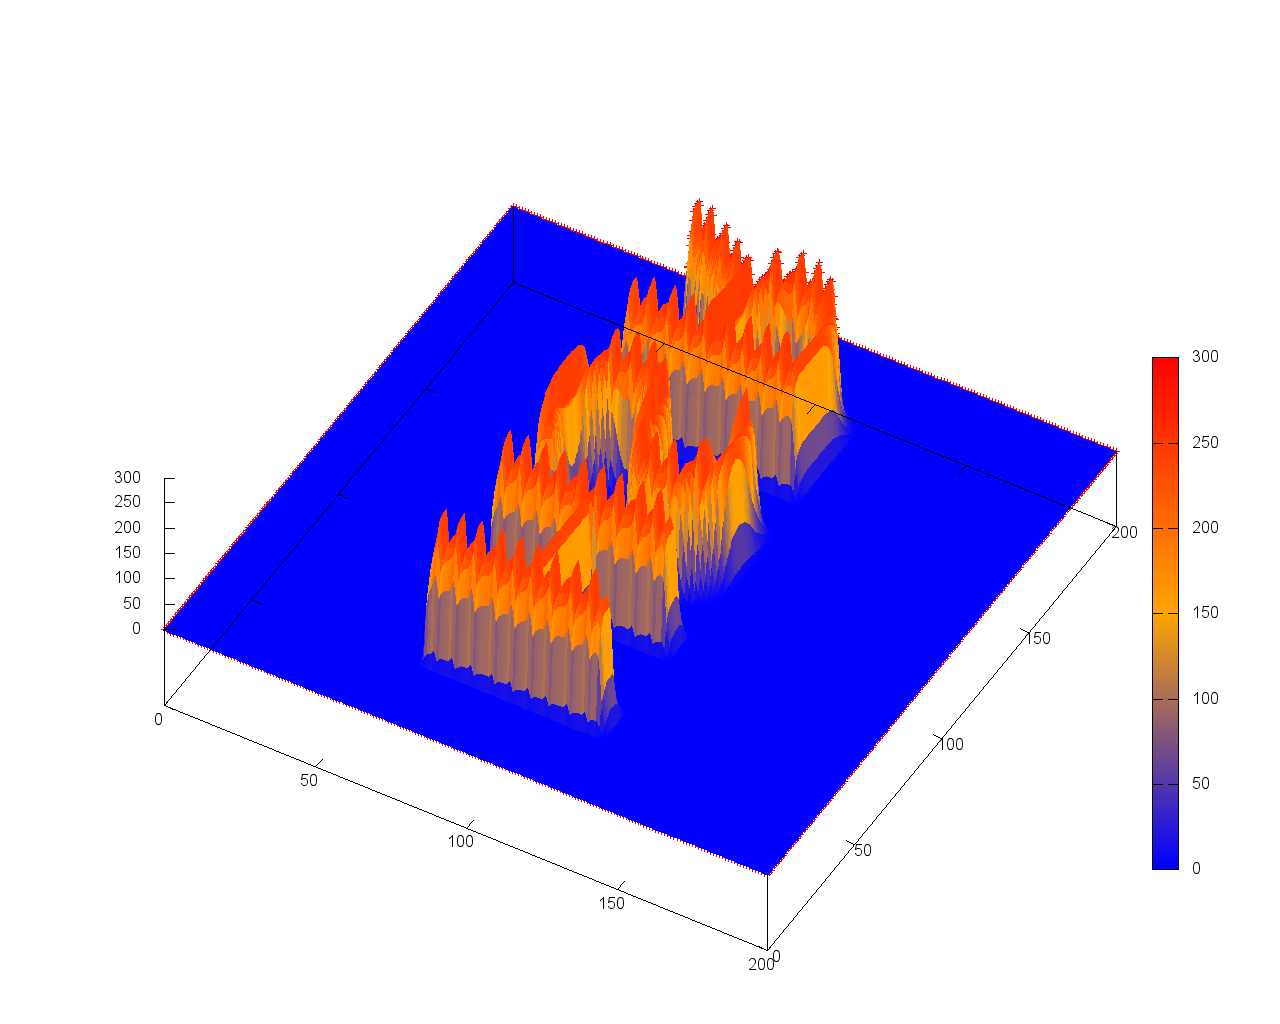
\includegraphics[width = 15cm]{./images/step001}
			\caption{Berechnung von einer $201 \times 201$ Fl�che mit 32 Threads nach dem ersten Iterationsschritt}
			\label{fig:201_1}
		\end{figure}
		
		
		Wir haben uns f�r OpenMP entschieden, da wir ein Grosses Problem haben, welches immer auf den selben Speicher zugreift. Wie schon beim Kugelsternhaufen erw�hnt, ist die Parallelisierung einfach zu realisieren:
		
\begin{code}
	int numthreads = 32;
	#pragma omp parallel for num_threads(numthreads)
		for (i = 0; i < dim; i++)
		{ ...
\end{code}
		
		
		
		

